\documentclass[10pt,a4paper]{report}
\usepackage[latin1]{inputenc}
\usepackage{amsmath}
\usepackage{amsfonts}
\usepackage{amssymb}
\usepackage{graphicx}
\author{Seth Bertlshofer\\Alexis Tyler\\Dustin Ginos\\Kevin Burgon}
\title{Desc. Experience 1}
\graphicspath{{img/}}
\begin{document}
	\maketitle
	\textbf{Sub-Experience One: Fun and Games}\\
		\begin{center}
			Figure 1.\\
			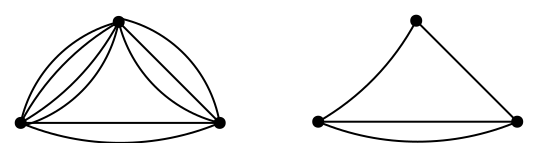
\includegraphics[scale=.5]{e1.png}
			\newline
			\newline
		\end{center}
		
	\textbf{Solution: }Player $A$ can always win if she employs a particular strategy for each move.  Let $G = (V, E)$ be a NIM graph where $x, y, z \in V$ ($V$ being the set of vertices in $G$) and $xy, yz, zx \in E$.  Assume that the graph never has the same number of edges between all vertices. The strategy that will be used is this: For each turn, player $A$ removes edges on one vertex such that $|xy| = |yz|$, $|yz| = |zx|$, and $|zx| = |xy|$, where $|E|$ is the number of edges between two vertices. Since the rule of the game is that the winner is the player who removes the last edge, we know that the winner is also the one who removes the second to last edge.  If that is the case, then the player who removes edge that breaks the cycle in the graph loses. The player that is forced to break the cycle is also the player who is forced to remove an edge such that either $|xy| = 1$, $|yz| = 1$, or $|zx| = 1$.  In order for player $A$ to force player $B$ to do that, player $A$ needs to force player $B$ to remove an edge from the pair of vertices with the minimum number of edges.  In order to do that, player $A$ needs to remove edges on every turn such that $|xy| = |yz|$, $|yz| = |zx|$, and $|zx| = |xy|$. Therefore, if the graph is such that $|xy| = |yz|$, $|yz| = |zx|$, and $|zx| = |xy|$, player $B$ is forced to remove edges until they break the cycle, and player $A$ will always win.\\
	
	%In that case, the strategy consists in leaving the graph such that player $B$ is forced to remove an edge that breaks the cycle.  In order to accomplish that the goal is also to force player $B$ to remove edges until they end a turn where $|xy| = 1$, $|yz| = 1$, or $|zx| = 1$.  In order to accomplish this player $A$ needs to avoid removing edges from the pair of vertices with the minimum number of edges.  If player $A$ never removes edges from the pair of vertices with the minimum number of edges player $B$ is forced to do so, therefore causing player $B$ to eventually remove an edge that results in a pair of vertices with only one edge between them.  In order for player $A$ to avoid  removing from the minimum number of edges, player $A$ always needs to remove edges such that $|xy| = |yz|$, $|yz| = |zx|$, and $|zx| = |xy|$.\\

	\textbf{Sub-Experience Two: The Binary Addressing Graph}
		\begin{enumerate}
			\item $|V(Q_n)| = 2^n$
			\begin{center}
				Figure 2.\\
				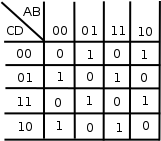
\includegraphics[scale=.5]{2_1.png}
			\end{center}
			Because this solution is looking for a binary power we can prove this with a Karnaugh Map (Figure 2) What this shows in the relation between the vertices.  If there is a relation then 1's will be adjacent to one another.  We can see that because the pattern is that is created by the Karnaugh map there can be no relations between vertices.
			\item $Q_n$ is an n-regular graph: that is, $deg (\vec{v}) = n $ for each $\vec{v} \epsilon V(Q_n)$.
			\item $Q_n$ is \textit{bipartite}; that is, $V(Q_n)$ consists of two sets, say X and Y such that $X\cap Y = \varnothing$ and the only edges of $Q_n$ have one end-vertex in X and the other in Y (so X and Y induce graphs with no edges).
			\item $Q_n$ is Hamiltonian for $n \geq 2$.
		\end{enumerate}
		
		
	\textbf{Sub-Experience Three: Space Station Problems}\\
	
		\begin{center}
			Figure 3.\\
			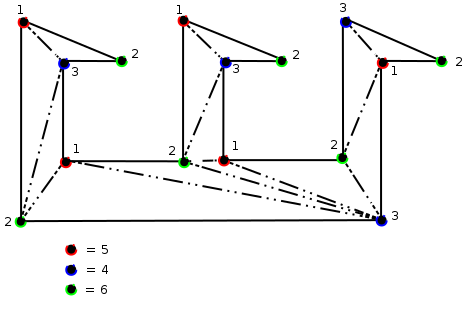
\includegraphics[scale=.5]{e3.png}
			\newline
			\newline
		\end{center}
	\textbf{Sub-Experience Four: Regions Determined by Chords of a Circle}\\
	
		\begin{center}
			%\includegraphics[scale=.5]{.png}
	
		\end{center}
	\textbf{Sub-Experience Five: Survivors in a Tournament.}\\
		As we look at Figure 4. This is the best way to explain how to prove this.  If we start making queens of 7 in the tournament (which is the least amount that any vertex can have to win) and work CW we end up with 3 queens. Now if we to to our original starting vertex and work CCW we find 2 more queens of 7.  We then end up with 5 queens after the first round.  Therefore, the max number of teams that will remain after the first elimination round will be 5.\\
		\newline
		For the second round if we keep the same pattern but with queens of 3 (which is the "majority" number to win) We will find that there ends up being 3 queens.Therefore, the max number of teams that will remain after the second round will be 3.\\
		\begin{center}
			Figure 4.\\
			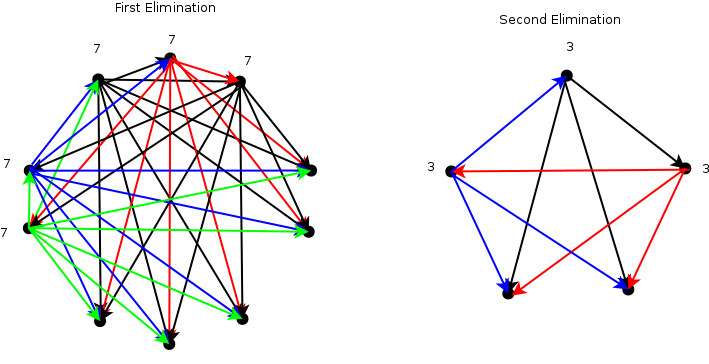
\includegraphics[scale=.5]{e5.png}
			\newline
			\newline
		\end{center}
	\textbf{Sub-Experience Six: Better-Than-Good Will Hunting}\\
		Verify that the graph G (below) has a diameter of 2.\\
		
		\noindent\textbf{Solution: }Using the given graph we make an adjacency matrix for all the vertices where <<CORRESPONDING VERTICES>>.  In meeting 25 we discussed that the power of an adjacency matrix theorem A: \emph{Suppose $G$ is a graph and $V(G) = \{v_{1}, v_{2}, ..., v_{n}\}$.  Then if $A$ is the adjacency matrix of $G$, entry $(i, j)$ in $A^{k}$ is the number of walks of length $k$ from $v_{i}$ to $v_{j}$.}.  The adjacenty matrix of this graph $G$ is  \\\\
		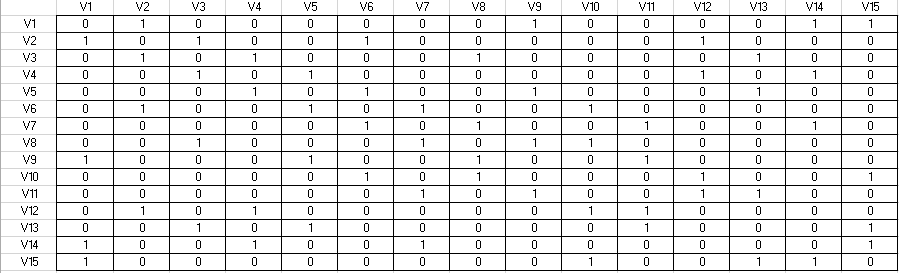
\includegraphics[scale=.64]{Math3310_Prob6.PNG} \\
		
		\noindent Therefore if we are to calculate $a^{2}$ we would get\\
		
		\noindent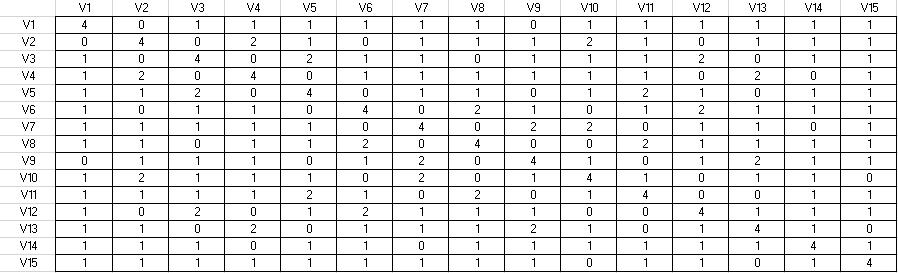
\includegraphics[scale=.64]{Math3310_Prob6-1.PNG}\\
		
		\noindent You can see that in matrix 2 all the cells that had a value of 0 in the first matrix now have a value equal to or greater than 1.  This means that there is a walk of 2 connecting any two nonadjacent vertices.  Therefore we can conclude that the maximum distance between any two vertices (aka the diameter) is 2.
		
		\begin{center}
			Figure 5.\\
			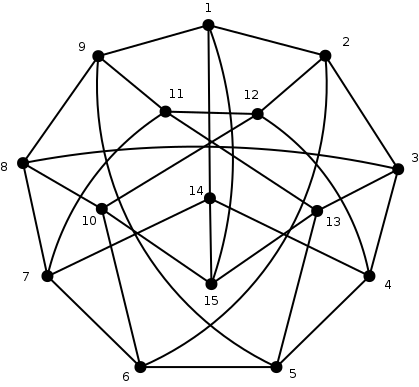
\includegraphics[scale=.5]{e6.png}
			\newline
			\newline
		\end{center}
	\textbf{[Bonus] Sub-Experience Seven: A Matter of Life and Death}\\	
		$n = 2^m + k$\\
		$w = 2k + 1$\\
		\textbf{w} = number of people in the group.\\
		\textbf{m} = the greatest exp. that can be without going over the \# of people with $(2^m)$ for example if w = 7 then m = 2 because $2^2 = 4$ if m = 3 then $7 = 2^3 = 8$ and it goes over the amount of people in the group.\\
		\textbf{k} = constant\\
		\textbf{n} = the spot that we want to stand not to die!\\
		\newline
		As we work through these formulas.  The 2nd formula is the first formula we need to look at.  It helps us find the k for the 1st formula.  Once we have that we can then find the exact spot we need to stand.\\
		\newline
		We can then plugin numbers now, if we have 13 people in the group.\\
		$13 = 2k + 1$ $k = 6$  Then $m = 3$ and $n = 2^3 + 6$ When will then need to stand in spot 14 in order not to die!
		\begin{center}
			%\includegraphics[scale=.5]{.png}

		\end{center}
\end{document}